\chapter{Návrh zařízení}

Tato kapitola se bude zabývat návrhem hardwaru celého zařízení. Jedním z~hlavních požadavků je nízká spotřeba, kterou bude třeba zohlednit při vybírání použitých senzorů, řídícího mikroprocesoru, komunikačního modulu a~ostatních obvodových komponent. 

\section{Výběr senzorů}
Celé zařízení bude schopno měřit koncentraci prachových částic, koncentraci oxidu uhelnatého, intenzitu osvětlení, intenzitu UV záření, teplotu, atmosférický tlak a~relativní vlhkost. V~následujících částech tedy bude popsán výběr z~dostupných senzorů.

\subsection{Senzor koncentrace prachových částic}

Na trhu je dostupných hned několik senzorů na měření koncentrace prachových částic. Jak již bylo zmíněno v~teoretickém úvodu, budu vybírat senzor, který tuto koncentraci určuje na základě osvícení daného vzorku vzduchu a~následně měření odraženého světla. Nyní vyvstává otázka, jestli zvolit senzor, který bude vzorek vzduchu vhánět do měřícího prostoru nuceně pomocí ventilátoru nebo jen za využití stoupání teplého vzduchu nahoru. V~tabulce \ref{tab_DustSensors} jsou uvedeny senzory, které jsou relativně cenově přijatelné, a~daly by se pro neprofesionální měření využít.

\newcommand{\ugcm}{\micro\gram\per\cubic\meter} % define new command used in '\SI' -> micro gram per cubic meter

\begin{table}[h]
    \centering
    \begin{tabular}{c|cccc}
    \textbf{Název}           & \textbf{Rozlišení}                & \textbf{Přesnost}                              & \textbf{Proud}                           & \textbf{Čas čtení}                \\ \hline
    \multirow{2}{*}{PMS5003} & \multirow{2}{*}{\SI{1}{\ugcm}}    & $0-100$\SI{}{\ugcm}:$\pm$\SI{10}{\micro\gram}  & \multirow{2}{*}{\SI{100}{\milli\ampere}} & \multirow{2}{*}{\SI{10}{\second}} \\
                             &                                   & $100-500$\SI{}{\ugcm}:$\pm$\SI{10}{\percent}   &                                          &                                   \\ \hline
    \multirow{2}{*}{PM1003}  & \multirow{2}{*}{\SI{1}{\ugcm}}    & $0-100$\SI{}{\ugcm}:$\pm$\SI{30}{\micro\gram}  & \multirow{2}{*}{\SI{90}{\milli\ampere}}  & \multirow{2}{*}{\SI{30}{\second}} \\
                             &                                   & $100-500$\SI{}{\ugcm}:$\pm$\SI{30}{\percent}   &                                          &                                   \\ \hline
    \multirow{2}{*}{PM1006}  & \multirow{2}{*}{neuvedeno}        & $0-100$\SI{}{\ugcm}:$\pm$\SI{20}{\micro\gram}  & \multirow{2}{*}{\SI{30}{\milli\ampere}}  & \multirow{2}{*}{\SI{8}{\second}}  \\
                             &                                   & $100-500$\SI{}{\ugcm}:$\pm$\SI{20}{\percent}   &                                          &                                   \\ \hline
    GP2Y1010AU0F             & \SI{0,5}{\volt}$/$\SI{100}{\ugcm} & záleží na ADC                                  & \SI{20}{\milli\ampere}                   & \SI{1}{\second}                           
    \end{tabular}
    \caption{Porovnání vybraných parametrů senzorů koncentrace prachových částic}
    \label{tab_DustSensors}
\end{table}

Po pečlivém prostudování jednotlivých parametrů jsem zvolil senzor PMS5003 od firmy PLANTOWER. Důležitým aspektem při výběru byla také cena tohoto senzoru, v~době vypracovávání této práce jej šlo pořídit za zhruba 350~Kč. Dalším důležitým parametrem byla spotřeba proudu v~aktivním stavu, na první pohled se může zdát, že oproti všem senzorům má spotřebu nejvyšší. Oproti PM1003 má však třetinový čas potřebný k~získání měřených dat, takže spotřebovává sice vyšší proud, ale po kratší časový úsek. PM1006 má spotřebu proudu zhruba třetinovou, ale vzorek měřeného vzduchu se do měřícího prostoru dostává pomocí sálání a~tak je nutné zajistit konstrukčně dostatečně a~správně dimenzované průduchy a~také konstantní polohu a~hlavně náklon senzoru, což by mohlo být v~praxi téměř nemožné, pokud má být zařízení používáno také ve volném prostranství. Poslední ze senzorů v~tabulce \ref{tab_DustSensors} má zdánlivě nejlepší výsledky. Bohužel se jedná pouze o~měřící modul samotný, který neobsahuje žádný ventilátor ani řídící logiku, je tedy třeba tyto věci zapojit a~konstrukčně vyřešit. Nejjednodušší na obvodové zapojení, a~i z~hlediska parametrů přesnosti nejlepší, se tak jeví již zmíněný senzor PMS5003. Senzor potřebuje pro svou funkci napájení \SI{5}{\volt}, a~komunikuje přes rozhraní UART.

\begin{figure}
    \centering
    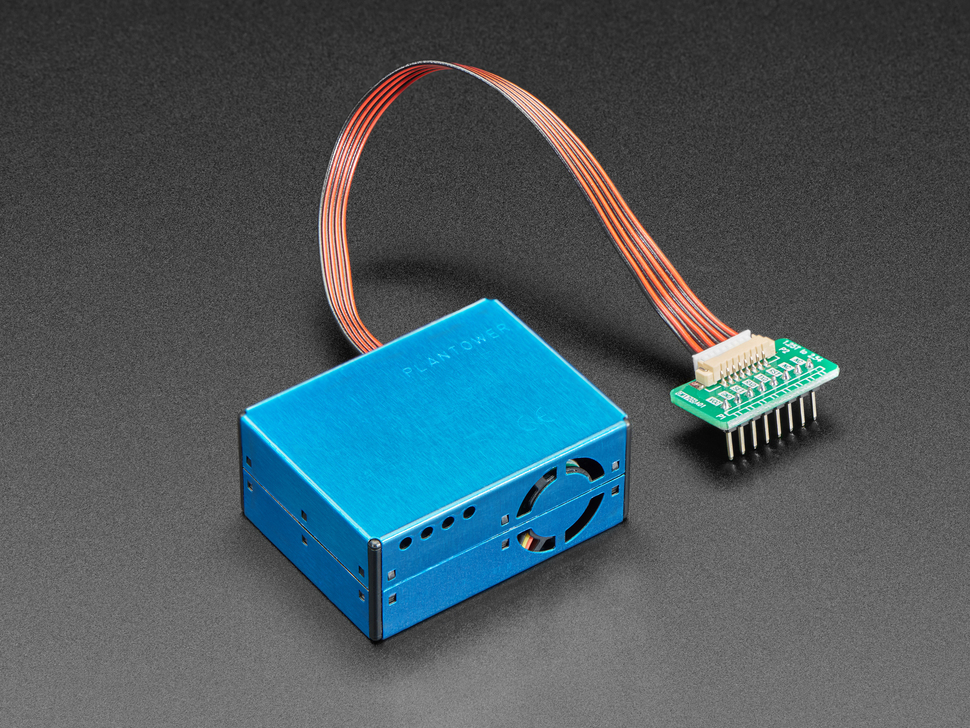
\includegraphics[width=0.7\textwidth]{obrazky/PMS5003.jpg}
    \caption{Senzor pro měření koncentrace prachových částic PMS5003. \cite{dat_PMS5003}}
    \label{fig_PMS5003}
\end{figure}

\subsection{Senzor oxidu uhelnatého}

U senzorů oxidu uhelnatého je situace o~něco složitější. Na trhu neexistuje mnoho možností, ze kterých by se dalo v~rozumné cenové kategorii vybírat. Pokud se podíváme do katalogů většiny (nejen českých) obchodů, zjistíme, že ceny čidel se pohybují ve vyšších stovkách korun až po několik tisíc. Tato cena je pro neprofesionální měření nepřijatelná. Jediným možným rozumným výběrem jsou čidla s~označením série MQ od výrobce Hanwei electronics\footnote{\url{https://www.hwsensor.com/}}. Vybral jsem tedy čidlo s~označením MQ-7, které je nejvíce citlivé právě na oxid uhelnatý. Funguje na principu ohřevu senzitivní vrstvy (zde konkrétně z~materiálu $SnO_{2}$) a~následně měření jejího odporu. Senzor je třeba napájet z~\SI{5}{\volt} a~jeho výstup je třeba přivést na AD převodník, jelikož má analogový výstup.

\begin{figure}
    \centering
    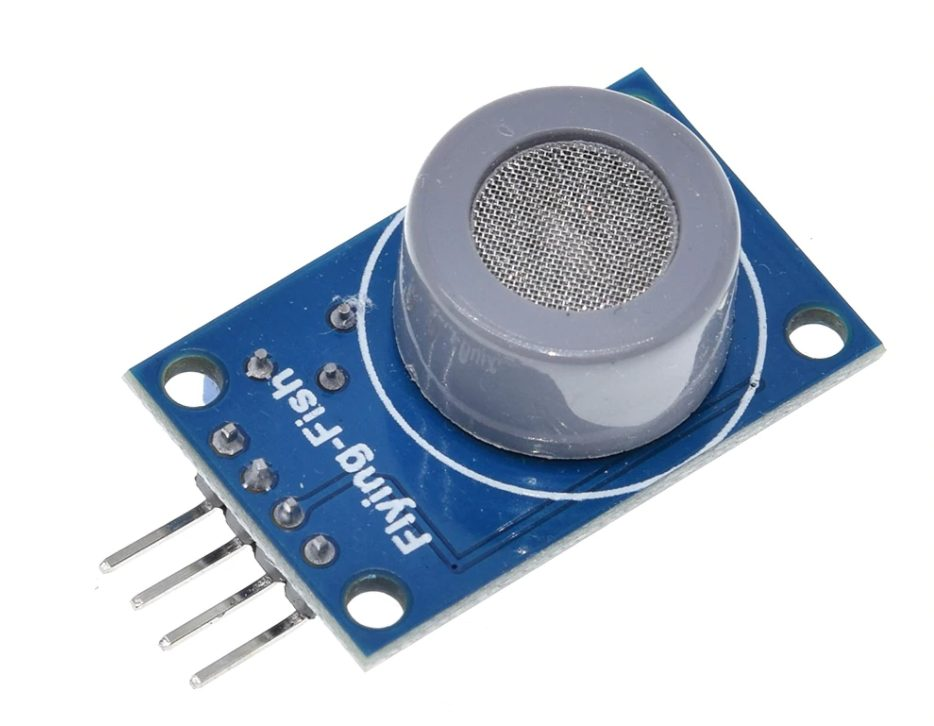
\includegraphics[width=0.7\textwidth]{obrazky/mq7.jpg}
    \caption{Senzor pro měření koncentrace oxidu uhelnatého. \cite{img_mq7}}
    \label{fig_MQ7}
\end{figure}

\subsection{Senzor UV záření}

Na poli relativně levných UV senzorů je výběr opět o~něco horší. Existují v~podstatě dvě varianty použitelné pro neprofesionální měření a~to senzor VEML6075 od výrobce VISHAY a~senzor ML8511 výrobce LAPIS Semiconductor. Bohužel první ze zmíněných senzorů se nedá rozumně sehnat, skladové zásoby jsou vyprodané a~několik obchodů udává, že se již nevyrábí.

Volím tedy druhý zmíněný senzor ML8511. Tento senzor měří pouze intenzitu UV záření pomocí fotodiody, která je citlivá na UVA a~UVB záření. Její největší citlivost je dle datasheetu \cite{dat_ML8511} na vlnovou délku \SI{365}{\nano\metre}. Pro svou činnost potřebuje napájení \SI{3,3}{\volt} a~během měření je jeho maximální spotřeba \SI{500}{\micro\ampere}. Pokud jej uvedeme pomocí pinu EN do režimu standby, tak může být spotřeba maximálně \SI{1}{\micro\ampere}. Výstup senzoru je opět napěťový, takže musíme jeho výstup přivést na AD převodník. Rozsah těchto napětí je zhruba od \SI{1}{\volt} do \SI{3}{\volt}, což odpovídá rozsahu \SI{0}{} až \SI{15}{\milli\watt\per\centi\metre\squared}

\subsection{Senzor teploty}

Na poli senzorů pro měření teploty existuje nepřeberné množství různých druhů od spousty výrobců. Pro první základní výběr vhodných senzorů je nutné si definovat alespoň základní parametry a~požadavky na takovýto senzor. Vhodnými parametry jsou cena, rozsah měřených teplot (je třeba měřit i~při teplotách nižších než \SI{0}{\celsius}), spotřeba a~přesnost. Srovnání potenciálně použitelných senzorů se nachází v~tabulce \ref{tab_TemperatureSensors}. Cena uvedená v~posledním sloupci je brána v~jeden den z~jednoho e-shopu\footnote{\url{https://www.laskarduino.cz/}}, aby bylo možné objektivně porovnat výsledky mezi sebou.

\begin{table}[]
    \centering
    \begin{tabular}{c|cccc}
    \textbf{Název} & \textbf{Rozsah}                         & \textbf{Přesnost}       & \textbf{Spotřeba}       & \textbf{Cena} \\ \hline
    DS18B20        & \SI{-55}{\celsius} - \SI{125}{\celsius} & $\pm$\SI{0,5}{\celsius} & \SI{1,5}{\milli\ampere} & 68~Kč         \\
    LM75A          & \SI{-25}{\celsius} - \SI{100}{\celsius} & $\pm$\SI{2}{\celsius}   & \SI{280}{\micro\ampere} & 25~Kč         \\
    SHT31          & \SI{-40}{\celsius} - \SI{90}{\celsius}  & $\pm$\SI{0,3}{\celsius} & \SI{350}{\micro\ampere} & 158~Kč        \\
    SHT35          & \SI{-40}{\celsius} - \SI{90}{\celsius}  & $\pm$\SI{0,2}{\celsius} & \SI{1,5}{\milli\ampere} & 378~Kč        \\
    SHT40          & \SI{-40}{\celsius} - \SI{125}{\celsius} & $\pm$\SI{0,2}{\celsius} & \SI{350}{\micro\ampere} & 109~Kč             
    \end{tabular}
    \caption{Srovnání parametrů vybraných senzorů teploty.}
    \label{tab_TemperatureSensors}
\end{table}

Z tabulky \ref{tab_TemperatureSensors} jsem nakonec pro svou práci vybral senzor SHT40 od výrobce SENSIRION. Bohužel není úplně nejlevnější, ale vybral jsem jej díky jeho nízké spotřebě \SI{350}{\micro\ampere} při měření a~až \SI{3,4}{\micro\ampere} v~nečinném stavu a~také relativně vysoké přesnosti, která je až \SI{0,2}{\celsius}. Napájení senzoru je \SI{3,3}{\volt}. S~mikroprocesorem senzor komunikuje pomocí sběrnice I$^2$C. 

\begin{figure}
    \centering
    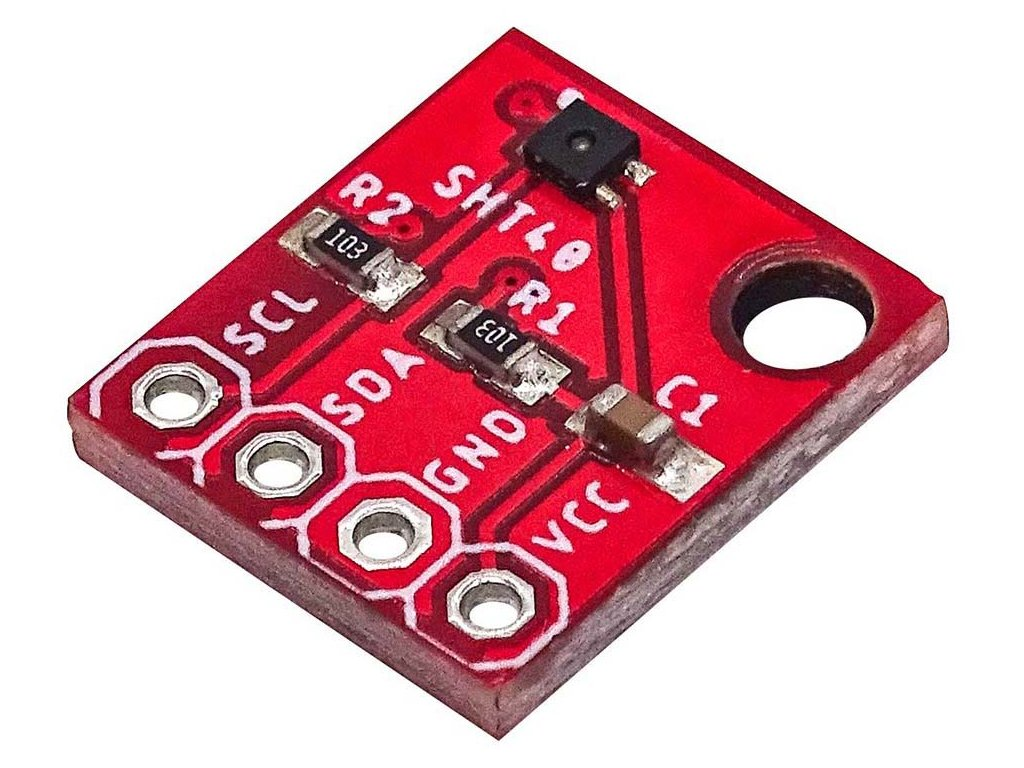
\includegraphics[width=0.55\textwidth]{obrazky/sht40.jpg}
    \caption{Senzor pro měření teploty SHT40. \cite{SHT40}}
    \label{fig_SHT40}
\end{figure}

\subsection{Senzor intenzity osvětlení}

Na poli senzorů pro měření intenzity osvětlení existuje hned několik dostupných variant. Liší se převážně způsobem, jakým intenzitu měří a~pak také rozsahem, pro které je možné jejich použití. Pro orientační měření lze využít i~prostého fotorezistoru, který zapojíme společně s~odporem do série a~vytvoříme si tak napěťový dělič, na kterém budeme měřiti pomocí AD převodníku analogové napětí. Tento typ měření je však silně závislý na použitém typu fotorezistoru a~většinou nebývá moc přesné. Využití této metody je spíše pro účely orientačního měření a~určení základních informací a~to, jestli je tma či jestli je světlo. 

Dalším z~možných typů senzorů je využití fototranzistoru nebo fotodiody. Toto měření je přesnější než předchozí zmíněná metoda, ale vyžaduje znalost přechodové charakteristiky součástky a~pro přesnější měření i~kalibraci vůči známé referenční hodnotě intenzity osvětlení.

Mnohem vhodnějším typem senzorů pro toto konkrétní použití je tak integrovaný senzor, který obsahuje jednak samotnou na světlo citlivou vrstvu a~druhak i~řídící logiku, která nám poskytuje digitální výstup ze senzoru například ve formě sériové sběrnice.

V tabulce \ref{tab_LuxIntensitySensors} jsou uvedeny vybrané druhy integrovaných senzorů a~jejich základní vlastnosti.

\begin{table}[h]
    \centering
    \begin{tabular}{c|cc}
        \textbf{Název} & \textbf{Rozsah}            & \textbf{Spotřeba}         \\ \hline
        GY-302 BH1750  & \SI{0}{}-\SI{65535}{\lux}  & \SI{200}{\micro\ampere}   \\
        TSL2561        & \SI{0}{}-\SI{40000}{\lux}  & \SI{0,6}{\milli\ampere}   \\
        VEML7700       & \SI{0}{}-\SI{120000}{\lux} & \SI{50}{\micro\ampere}
    \end{tabular}
    \caption{Srovnání parametrů vybraných senzorů intenzity osvětlení.}
    \label{tab_LuxIntensitySensors}
\end{table}

Z těchto vybraných dostupných senzorů jsem zvolil poslední z~tabulky VEML7700. Tento senzor má velmi nízkou spotřebu i~při nejrychlejším cyklu čtení (\SI{100}{\milli\second}) a~největší rozsah možného měření. Při porovnání cen se nachází zhruba ve stejné cenové hladině jako druhý nejlepší z~této tabulky GY-302~BH1750. S~mikrokontrolerem senzor bude komunikovat pomocí sběrnice I$^2$C a~napájen bude z~\SI{3,3}{\volt}.

\begin{figure}[h!]
    \centering
    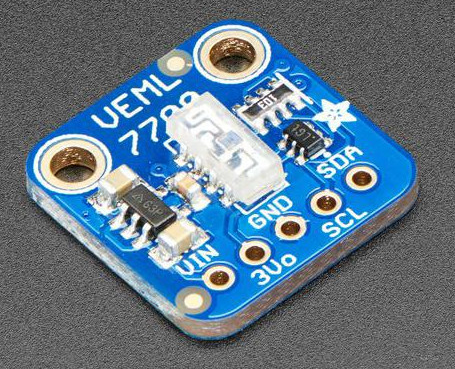
\includegraphics[width=0.4\textwidth]{obrazky/veml7700.png}
    \caption{Senzor pro měření intenzity osvětlení VEML7700. \cite{VEML7700}}
    \label{fig_VEML7700}
\end{figure}

\subsection{Senzor atmosférického tlaku}

Posledním z~potřebných senzorů je senzor pro měření atmosférického tlaku. Existuje několik senzorů, které integrují do jednoho pouzdra měření teploty, vlhkosti i~atmosférického tlaku. Tyto senzory se však vyznačují nižší přesností. Jedním z~takovýchto senzorů je například BME280 od výrobce Bosch, který je populární mezi kutily při stavění amatérské domácí meteostanice. Bohužel poslední dobou není dostupný skladem v~žádném z~velkých obchodů a~pokud se někde vyskytne, stojí několikanásobek jeho normální ceny a~je tak pro tuto práci nepoužitelný.

Budu tedy porovnávat senzory, které měří pouze atmosférický tlak a~jsou dostupné a~mají relativně nízkou cenu.

\begin{table}
    \centering
    \begin{tabular}{c|ccc}
        \textbf{Název} & \textbf{Rozsah}                     & \textbf{Přesnost}      & \textbf{Spotřeba}        \\ \hline
        BMP180         & \SI{300}{}-\SI{1100}{\hecto\pascal} & $\pm$\SI{3}{\pascal}   & \SI{12}{\micro\ampere}   \\
        BMP280         & \SI{300}{}-\SI{1100}{\hecto\pascal} & $\pm$\SI{1,3}{\pascal} & \SI{2,7}{\micro\ampere}  \\
        BMP388         & \SI{300}{}-\SI{1250}{\hecto\pascal} & $\pm$\SI{8}{\pascal}   & \SI{3,4}{\micro\ampere}  \\
        BME280         & \SI{300}{}-\SI{1100}{\hecto\pascal} & $\pm$\SI{2}{\pascal}   & \SI{7,1}{\micro\ampere}  \\
        ICP-10100      & \SI{300}{}-\SI{1150}{\hecto\pascal} & $\pm$\SI{3,2}{\pascal} & \SI{10,4}{\micro\ampere} 
    \end{tabular}
    \caption{Srovnání parametrů vybraných senzorů atmosférického tlaku.}
    \label{tab_AirPressureSensors}
\end{table}

Jak je uvedeno v~tabulce \ref{tab_AirPressureSensors}, je vidět že většina senzorů atmosférického tlaku je od výrobce Bosch Sensortec. Vyskytuje se zde již zmiňovaný BME280, který je ale moc drahý a~momentálně nedostupný a~při měření tlaku má jednu z~vyšších spotřeb. Dalším ideálním adeptem by byl i~senzor BMP280, který umožňuje měřit atmosférický tlak i~teplotu. Bohužel ani tento senzor není příliš dostupný a~dle oficiálních stránek výrobce již není doporučen pro nové návrhy.

Vybral jsem tedy senzor BMP388 od firmy Bosch Sensortec. Nepatří bohužel mezi nejlevnější, ale zato je dostupný v~obchodech a~poskytuje vzhledem ke své dostupnosti relativně dobré parametry samotného měření. Stejně jako dříve zmíněné senzory, i~tento senzor umožňuje kromě atmosférického tlaku měřit i~teplotu. Pro komunikaci s~mikrokontrolerem lze použít sběrnici I$^2$C nebo SPI, jelikož je většina vybraných senzorů na sběrnici I$^2$C, použiji stejnou sběrnici i~pro tento senzor. Napájení je třeba přivést \SI{3,3}{\volt}.

\subsection{Senzor měření vlhkosti}

Jak již bylo zmíněno v~kapitole o~výběru senzoru pro měření teploty, vybraný senzor SHT40 umožňuje měřit i~vzdušnou vlhkost. Rozsah měření je \SI{0}{}-\SI{100}{\percent} relativní vlhkosti s~přesností $\pm$\SI{1,8}{\percent}. Pro potřeby měření relativní vzdušné vlhkosti v~této práci jsou tyto parametry s~přehledem dostatečné.

\section{Výběr řídícího mikrokontroléru}

Mikrokontroler je hlavním řídícím prvkem celého zařízení. Při jeho výběru je nutné dbát na spousty mnohdy protichůdných parametrů. Jedním z hlavních a~nejdůležitějších parametrů jsou požadavky na hardwarové periferie a~celkově výbavu daného mikrokontroleru. Jak již bylo popsáno v předchozích kapitolách této práce, je nutné všechny senzory připojit pomocí různých sběrnic či zajistit AD převodník pro připojení analogových výstupů ze senzorů. Také je třeba dbát na dostatečný počet vstupně-výstupních pinů.

V dnešní době má spousta mikrokontrolerů přímo v sobě integrovanou rádiovou část, takže jsou schopny se připojit např. na WiFi, komunikovat s~ostatními zařízeními přes Bluetooth či posílat zprávy přes LoRa síť. Toto řešení zjednodušuje návrh výsledného zařízení a~také dokáže snížit výrobní náklady, jelikož je vše obsaženo v jednom čipu a~není třeba osazovat několik samostatných čipů. Zároveň snižuje pravděpodobnost chybného návrhu nebo eliminuje další možný zdroj poruch, jelikož každý další použitý čip na desce a~spojení k němu je možným zdrojem problémů.

Pro výběr v této práci budu uvažovat výběr mikrokontrolerů od největších výrobců jako jsou STMicroelectronics, Atmel (dnes Microchip) nebo Espressif Systems. Existuje samozřejmě spousta dalších výrobců, ale tihle uvedení jsou jedni z největších, nejznámějších a~nejdostupnějších. Porovnání ceny v tabulce \ref{tab_MCU} je provedeno v jeden den z jednoho obchodu\footnote{\url{https://www.tme.eu/cz/}} pro možnost objektivního posouzení. Do tabulky pro srovnání jsem vybral pouze nejdůležitější parametry daných mikrokontrolerů jako jsou hardwarové periferie pro sběrnice, počet GPIO (vstupně-výstupních pinů), přítomnost WiFi rozhraní a~cenu.

\begin{figure}[h]
    \centering
    \begin{tabular}{c|cccccc}
        \textbf{Název}                         & \textbf{I$^2$C} & \textbf{SPI} & \textbf{GPIO} & \textbf{USART} & \textbf{WiFi} & \textbf{Cena} \\ \hline
        ATmega328P \cite{dat_ATmega328p}       & 1 & 1 & 23 & 1 & Ne  & 70~Kč \\
        ESP32 WROOM \cite{dat_ESP32-WROOM}     & 2 & 4 & 34 & 3 & Ano & 80~Kč \\
        ATSAM4LC2 \cite{dat_ATSAM4LC2}         & 2 & 1 & 27 & 3 & Ne  & 90~Kč \\
        STM8L162R8T6 \cite{dat_STM8L162R8T6}   & 1 & 2 & 54 & 3 & Ne  & 110~Kč \\
        STM32L051C8T6 \cite{dat_STM32L051C8T6} & 2 & 2 & 37 & 2 & Ne  & 180~Kč
        
    \end{tabular}
    \caption{Srovnání parametrů vybraných mikrokontrolerů.}
    \label{tab_MCU}
\end{figure}

Z výše uvedené tabulky \ref{tab_MCU} jsem nakonec vybral mikrokontroler ESP32~WROOM od výrobce Espressif Systems. Z hlediska ceny není nejlevější, ale pokud se podíváme na parametry, které za tuto cenu nabízí, tak je to bezkonkurenční nabídka. Mikrokontroler samotný obsahuje kromě výše zmíněných parametrů i~rádiovou část ve které je obsažena WiFi a~Bluetooth, takže pro bezdrátové spojení není třeba použít žádný další modul. Mikrokontroler běží až na frekvenci \SI{240}{\mega\hertz} a~obsahuje dvě jádra, takže je možné velmi ryhle paralelně zpracovávat data. Mikrokontroler samotný je navržen pro IoT aplikace, takže je dbáno na velmi nízkou spotřebu při práci i~v mnoha režimech spánku, které je možné aktivovat. Hlavní dvě jádra mikrokontroleru jsou doplněna o tzv. ULP (Ultra Low Power) koprocesor, který je možné aktivovat v režimu spánku a~vykonávat tak velice jednoduché sekvence příkazů a~ovládat například výstupní piny. Na obrázku \ref{fig_ESP32InternalStructure} je vidět blokové schéma struktury mikroprocesoru ESP32 včetně všech jeho hardwarových periferií. Celý mikrokontroler je třeba napájet napětím \SI{3,3}{\volt} a~zdroj musí být schopen dodat alespoň \SI{500}{\milli\ampere}, tato hodnota je relativně vysoká, ale je to způsobeno potřebou vyššího příkonu při vysílání přes WiFi.

\begin{figure}
    \centering
    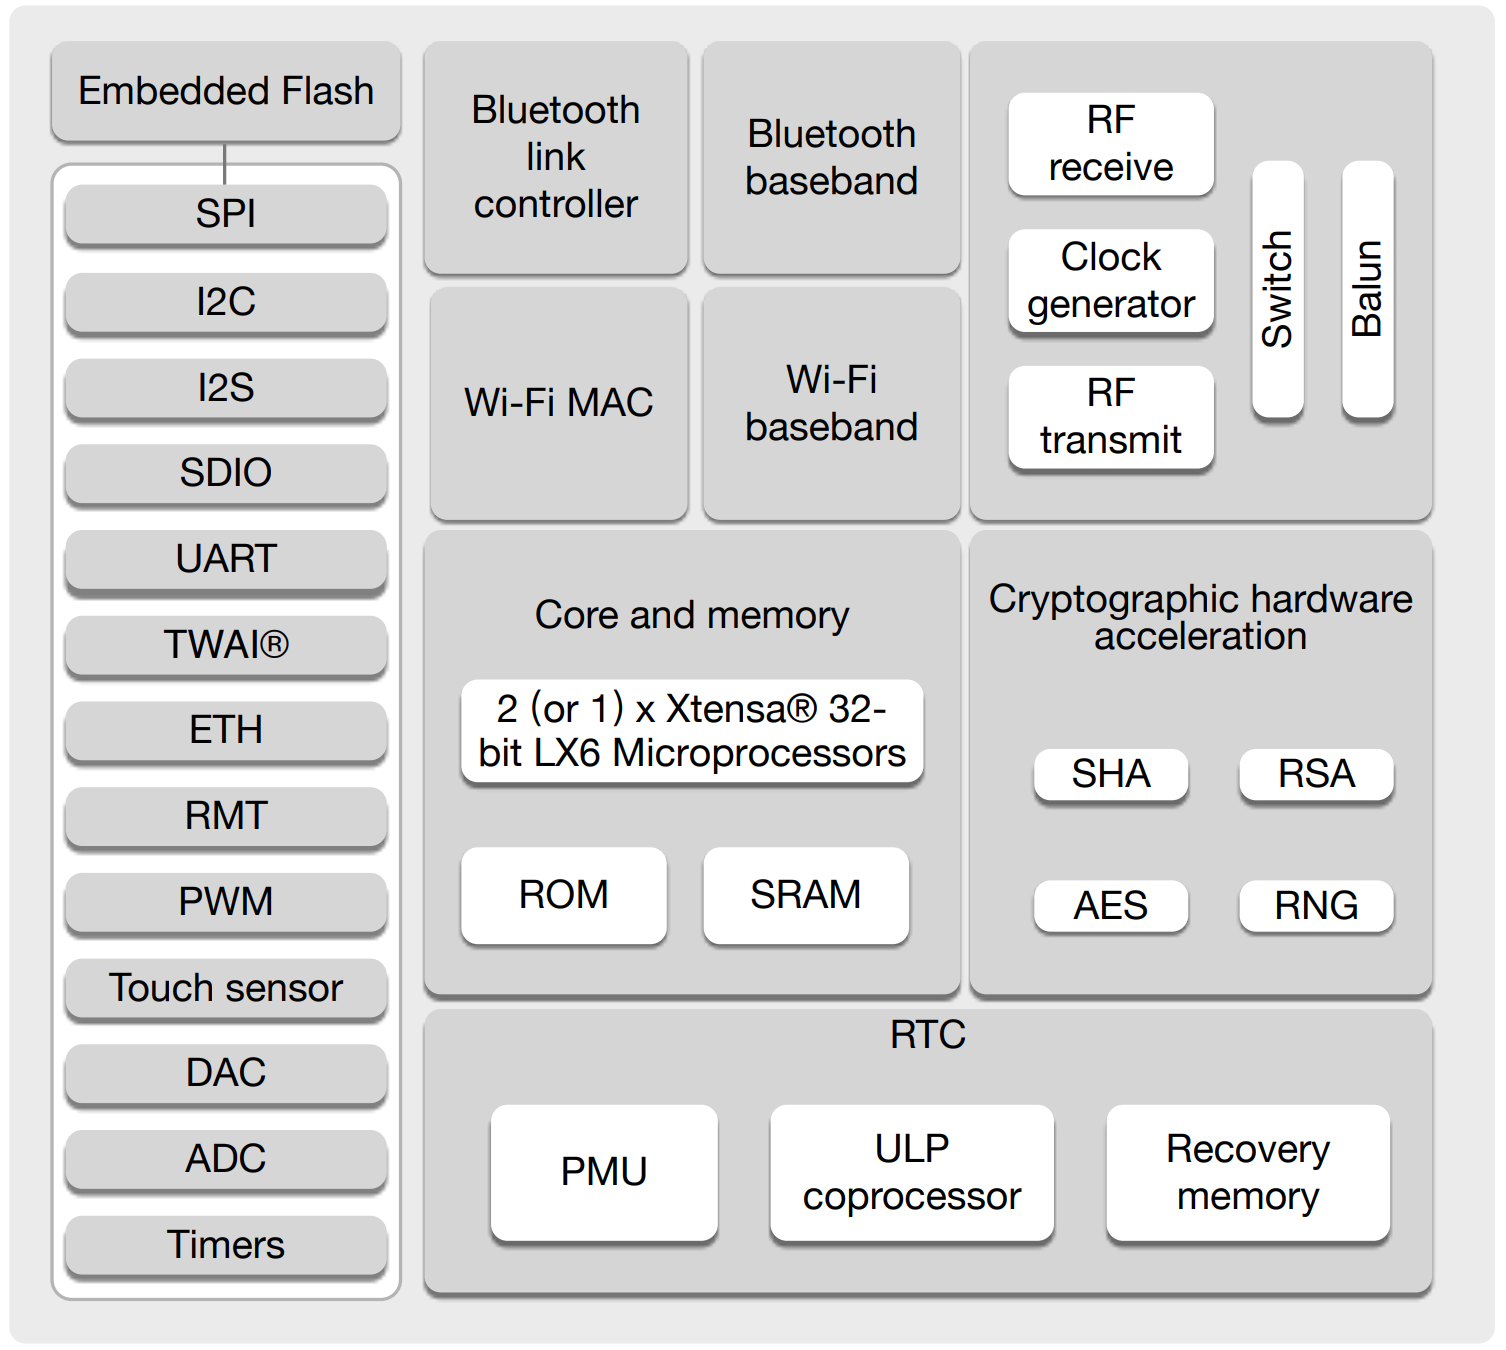
\includegraphics[width=0.7\textwidth]{obrazky/esp32_internalStructure.png}
    \caption{Blokový diagram mikrokontroleru ESP32.\cite{dat_ESP32-WROOM}}
    \label{fig_ESP32InternalStructure}
\end{figure}

\subsection{Analogově digitální převodník}

Jak již bylo zmíněno v předchozích kapitolách o výběru senzorů, bude potřeba zajistit analogové vstupy na mikrokontroleru. Bohužel ESP32 nemá příliš přesný AD převodník a je třeba provádět poměrně náročnou kalibraci pro každý zakoupený čip zvlášť, jak je zmíněno přímo v oficiální dokumentaci\footnote{https://docs.espressif.com/projects/esp-idf/en/latest/esp32/api-reference/peripherals/adc.html}. Nelze provádět ani kalibraci na jednom daném vzorku pro danou výrobní sérii.

Kvůli těmto výše uvedeným důvodům jsem se rozhodl pro tuto práci využít externí AD převodník, čímž by se měla zvýšit přesnost měření a zajistit reprodukovatelné výsledky při použití jiného mikrokontroleru. Hlavním požadavkem na výběr tohoto převodníku byla cena, dostupnost a spotřeba. Pro tuto práci je zapotřebí převodník, který bude moci být napájen z \SI{3,3}{\volt} a bude mít alespoň 2 vstupní kanály. Těmto požadavkům nejlépe vyhověl AD převodník MCP3202 od firmy Microchip Technology Inc.\cite{dat_MCP3202}. Obsahuje dva kanály s rozlišením 12 bitů. Připojení k mikrokontroleru je provedeno přes sběrnici SPI a maximální spotřeba při čtení je \SI{550}{\micro\ampere} při \SI{5}{\volt} napájení.

\section{Přenos dat na server}

Pro přenos naměřených dat na server je k dispozici celá řada možností, jak to provést. Jelikož budou data zpracovávána na serveru, který je dostupný přes síť internet, je třeba zajistit, aby se tam data dostala. Pro první pokusy bude nejjednodušší použití sítě WiFi, do které se se zařízením lze jednoduše připojit a poté se lze připojit na zpracovávatelský server. Toto řešení je ovšem nevhodné pro použití kdekoliv mimo obydlené oblasti či oblasti, kde máme pokrytí svou vlastní WiFi, protože se nelze spoléhat na to, že v daném místě potřeby bude nějaká např. veřejná síť. Další z nevýhod této technologie je její relativní energetická náročnost, jelikož je třeba vysílat na frekvenci \SI{2,4}{\giga\hertz} a po připojení musí zařízení získat IP adresu, což nějakou dobu trvá a poté může teprve probíhat komunikace. Jelikož však síť internetu a její protokoly nejsou uzpůsobeny na redukci datového toku, je celý přenos výrazně delší než vyslání zprávy např. přes síť LoRaWAN, což má opět negativní dopad na spotřebu energie.

Z výše uvedených důvodů se hodí využití jiné sítě, která je pro tato IoT zařízení přizpůsobená, je méně energeticky náročná a umožňuje připojení zařízení na řádově větší vzdálenosti. Jako nejjednodušší se jeví použití sítě LoRa. Pro tuto síť existuje na trhu mnoho komunikačních modulů, které jsou i relativně cenově přijatelné. Síť jako taková není zatížena licenčními poplatky, je však možnost využití již existující infrastruktury od nějaké firmy (u nás například České Radiokomunikace a.s.\footnote{https://www.cra.cz/pripojeni-k-iot-siti-lorawan}) kde se poté platí poplatky za využívání připojení k jejich síti či případné další služby.

Pokud chceme připojit zařízení přes LoRaWAN, ale nechceme být zavázání poskytovateli služeb a platit poplatky, je možnost použít některou z dostupných sítí, které jsou zdarma. Většinou se zde vyskytují omezení např. v počtu přenesených zpráv za daný čas nebo počet připojených zařízení. Jednou z nejznámějších sítí je TTN (The Things Network\footnote{https://www.thethingsnetwork.org/}). Princip této sítě je postaven na infrastruktuře, kterou do sítě připojují samotní uživatelé a tato služba je koncentruje na jeden server. Uživatelé tak mají možnost připojovat svoje vlastní gateway a poté libovolně v dosahu jakékoli jiné gateway připojené do sítě přenášet data ze svých zařízení.

\subsection{Výběr LoRa modulu}

Pro výběr LoRa modulu bude nejdůležitějším parametrem cena a dostupnost. Na našem území je dle ČTÚ a její národní kmitočtové tabulky\cite{kmitoctovaTabulka} povoleno provozovat LoRa zařízení v ISM pásmu \SI{868}{MHz}. Toto je také třeba zohlednit při výběru vhodného modulu. Dalším z kritérií byla dostupnost kvalitní dokumentace a také jestli existují příklady k použití daného modulu.

\DeclareSIUnit \belm {Bm}   %% declaration of Bel upper the milliwatt unit
Daným kritériím bezesporu vyhověl modul s označením RFM95W \cite{dat_RFM95W}, založený na čipu RF96. Jak již bylo zmíněno, modul pracuje na frekvenci \SI{868}{\mega\hertz} a nejvyšší možný výkon vysílače je \SI{20}{\deci\belm}. Modul pro své fungování potřebuje napájení \SI{3,3}{\volt} a při běžném vysílání výkonem \SI{+7}{\deci\belm} a dokonale přizpůsobené anténě na impedanci \SI{50}{\ohm} je jeho spotřeba \SI{20}{\milli\ampere}. Pro připojení k mikrokontroleru je zapotřebí sběrnice SPI a alespoň 1 GPIO (ideálně s podporou interruptu), jelikož modul umožňuje při přijetí dat ze sítě změnit logickou hodnotu na tomto pinu a tím dát hlavnímu mikrokontroleru vědět, že má přijatá data přečíst a zpracovat. 

\begin{figure}
    \centering
    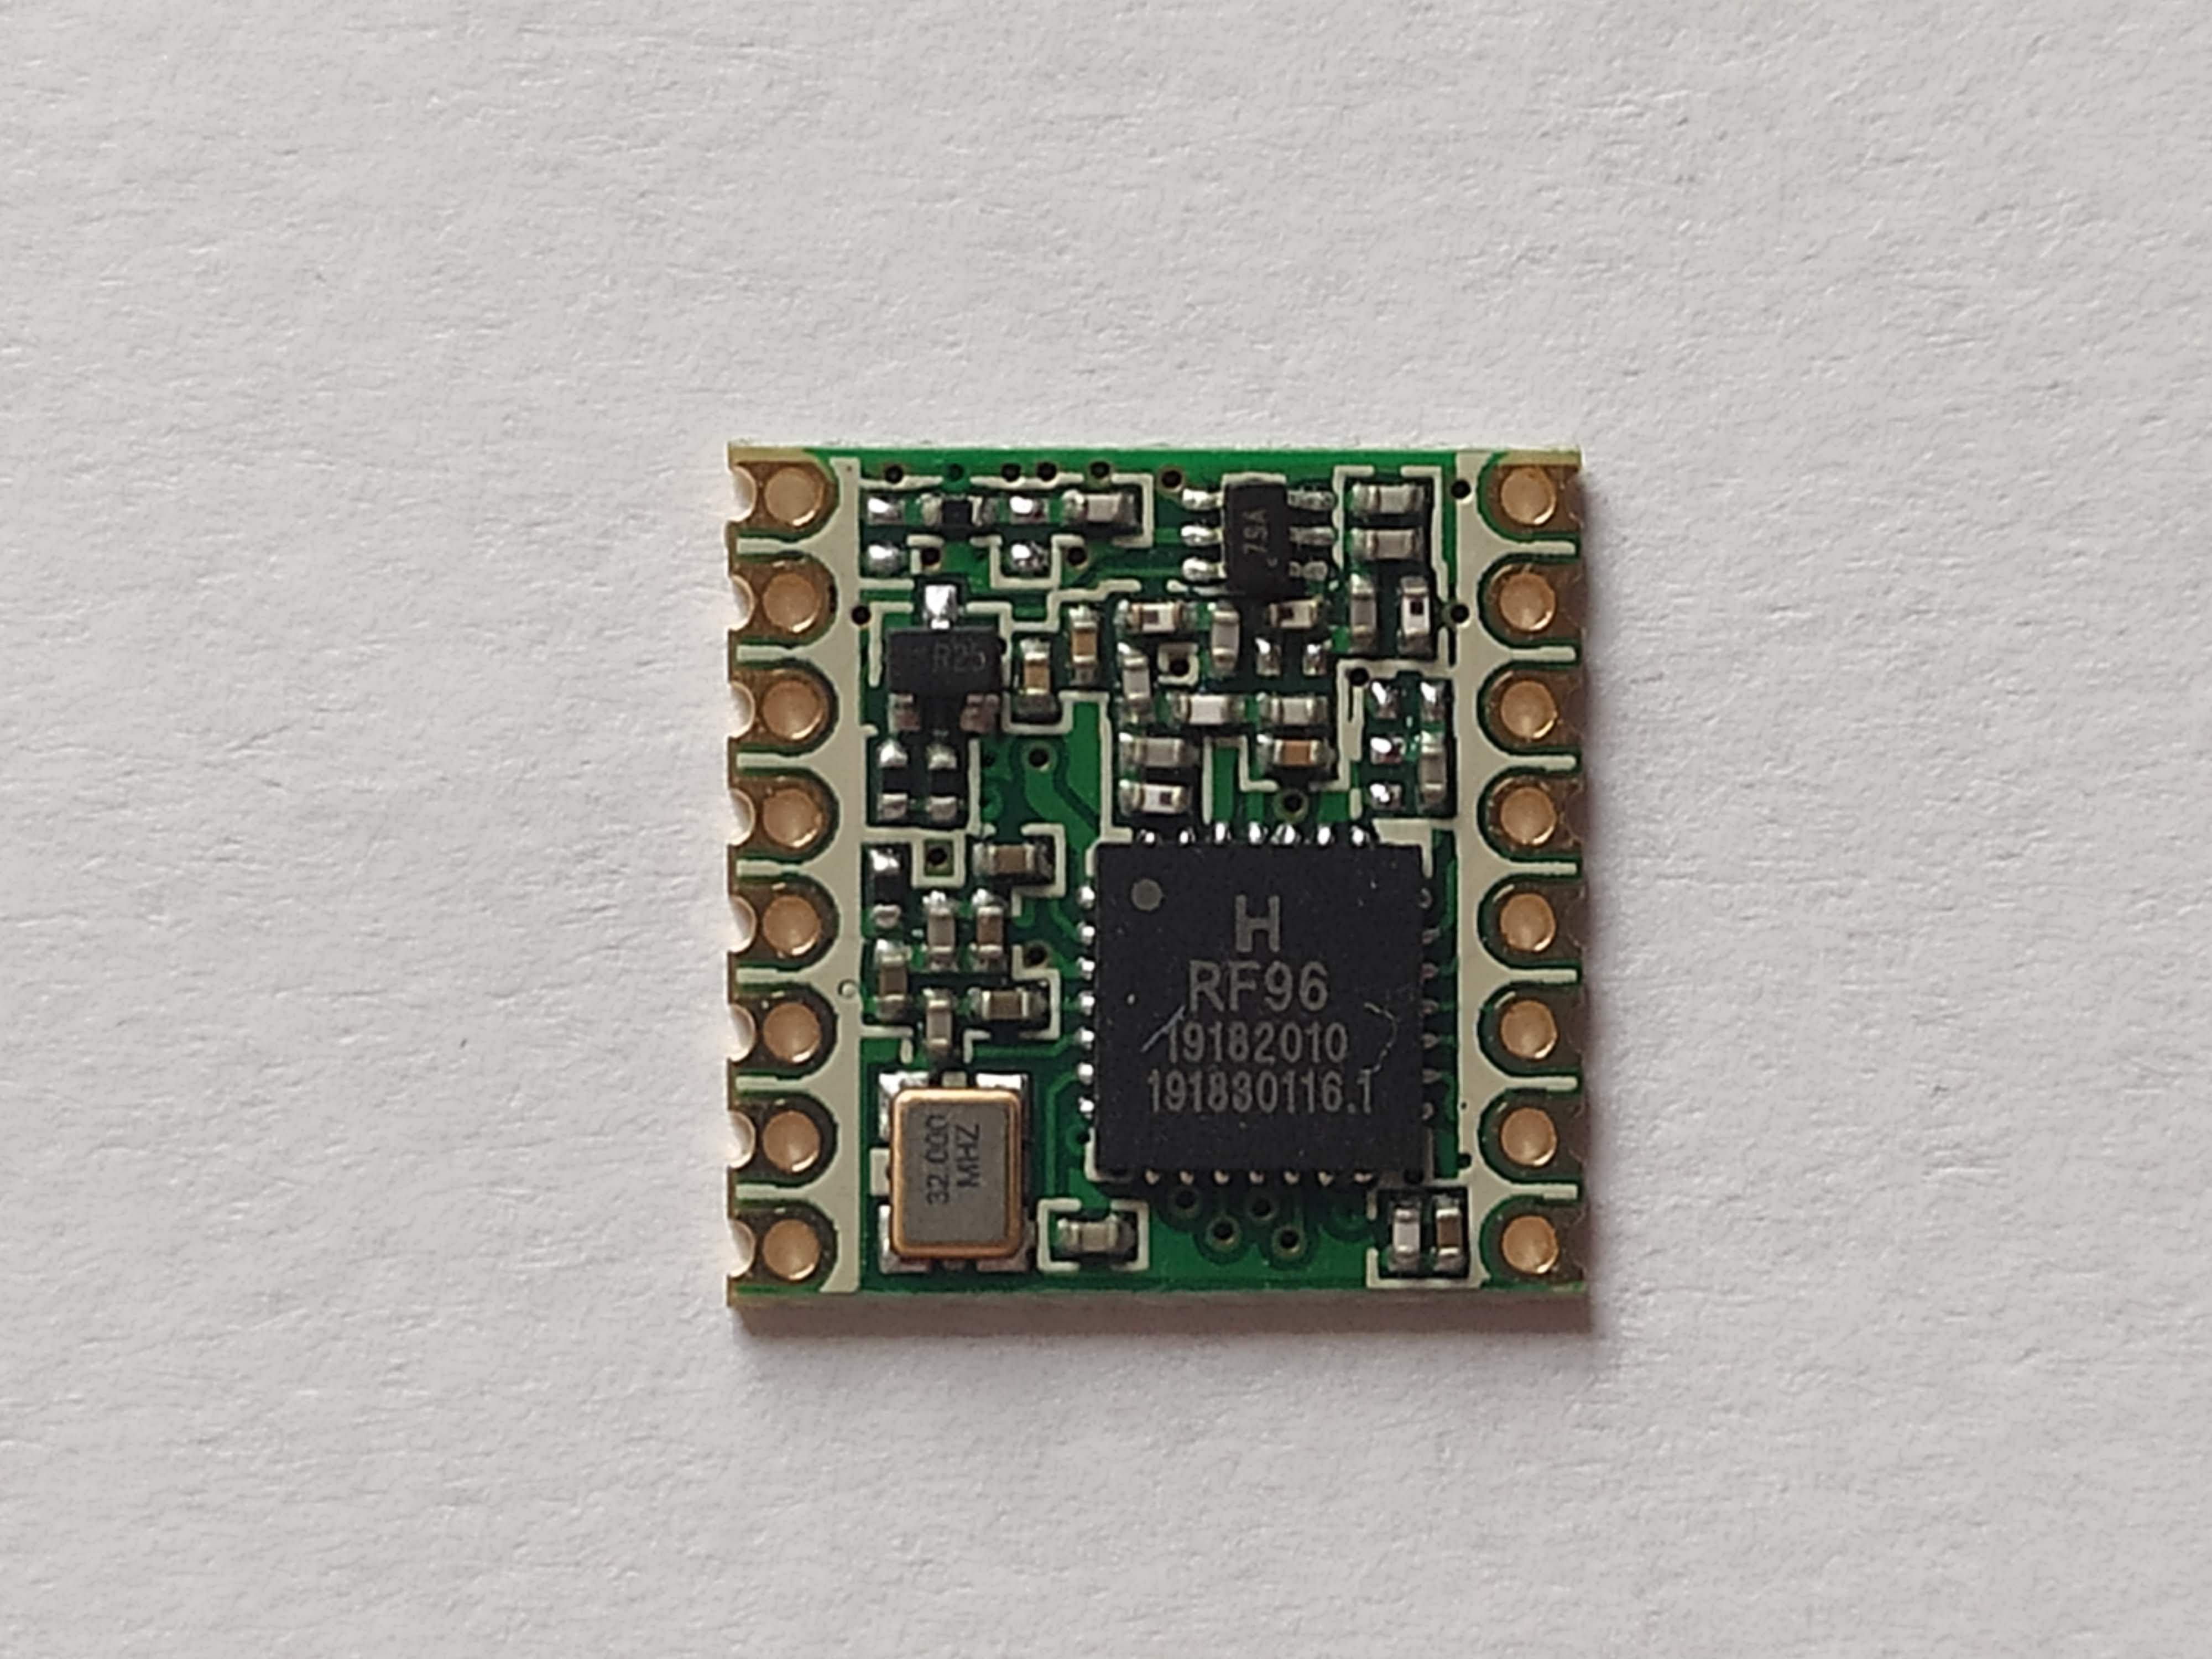
\includegraphics[width=0.7\textwidth]{obrazky/rfm95w.jpg}
    \caption{LoRa modul RFM95W.}
    \label{fig_RFM95W}
\end{figure}

\section{Napájení zařízení}

První verze tohoto zařízení bude napájena z \SI{5}{\volt} a bude tak možné využít např. mobilní nabíječky či powerbanky. Výhoodu tohoto řešení je zaručený zdroj napětí \SI{5}{\volt} a odpadá také nutnost například hlídání stavu baterií nebo řízení jejich nabíjení. V budoucích verzích ovšem chci zařízení napájet právě z baterií, aby odpadla nutnost mít k dispozici elektrickou rozvodnou síť a aby zařízení bylo použitelné kdekoli.

Celé zařízení ke své funkci tedy potřebuje napětí \SI{5}{\volt} a \SI{3,3}{\volt}. První ze zmíněných napětí bude bráno přímo ze zdroje (nabíječka nebo powerbanka) a není třeba se o něj více starat, jelikož tyto zařízení mají integrované různé druhy ochran (přepětí, nadrpoudová aj.). Je tedy třeba zajistit napájecí zdroj poskytující napětí \SI{3,3}{\volt}. Pro tyto účely bude třeba použít tzv. step-down měnič. Jelikož bude použit také externí AD převodník, je vhodné mu zajistit napájecí napětí, které nebude zatíženo zvlněním či jinými neduhy danými spínaným měničem. Z tohoto důvodu bude pro jeho napájení použit lineární stabilizítor. Protože je však rozdíl mezi vstupním napětím (\SI{5}{\volt}) a potřebným výstupním napětím (\SI{3,3}{\volt}) nižší než \SI{2}{\volt}, je třeba použít tzv. LDO (Low Dropout) lineární stabilizátor.

\subsection{Výběr step-down měniče}

Step-down měničů existují na trhu stovky různých druhů od všemožných výrobců. Výběr je tedy nutné provést převážně na základě potřebných parametrů jako jsou vstupní napětí, výstupní napětí a potřebný dodávaný proud. Jelikož je celé zařízení koncipováno jako nízkopříkonové, je vhodné podívat se také na výrobcem udávaný proud potřebný pro provoz samotného měniče. nejdůležitějším parametrem je bohužel v dnešní době dostupnost daného měniče a také jeho cena.

Já jsem pro svou práci vybral step-down měnič TPS54331 od výrobce Texas Instruments Incorporated\cite{dat_TPS54331}. Tento měnič lze používat až do vstupního napětí \SI{28}{\volt} a odebírat z něj výstupní proud \SI{3}{\ampere}. Díky tomu, že měnič obsahuje výkonový spínací tranzistor, tak není potřeba příliš mnoho externích součástek. Na obrázku \ref{fig_Schematic-TPS54331} je vidět zjednodušené zapojení tohoto měniče.

\begin{figure}
    \centering
    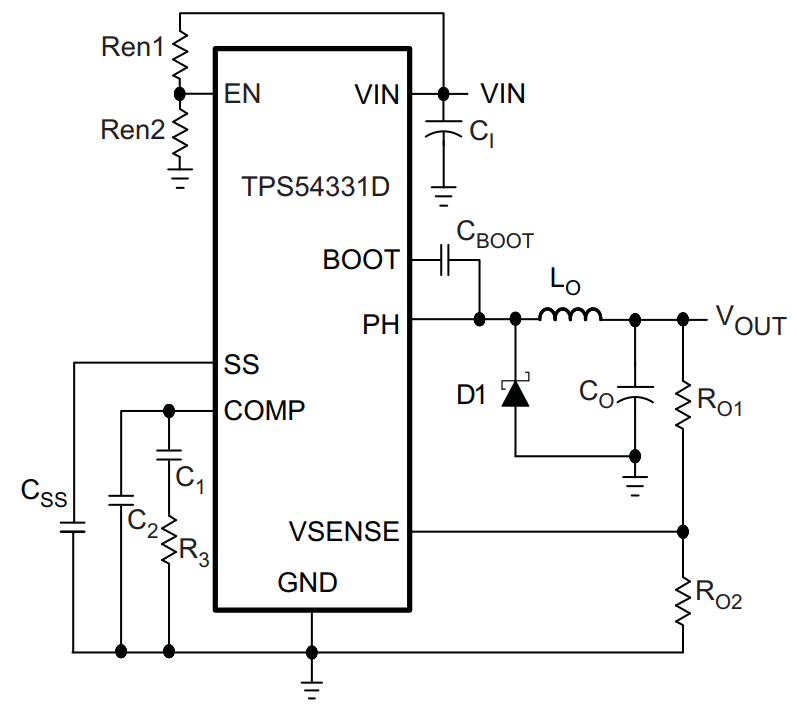
\includegraphics[width=0.6\textwidth]{obrazky/schematicTPS54331.png}
    \caption{Zjednodušené schéma zapojení měniče TPS54331.\cite{dat_TPS54331}}
    \label{fig_Schematic-TPS54331}
\end{figure}

\subsubsection{Návrh hodnot součástek step-down měniče}

Při návrhu součástek budu vycházet z datasheetu poskytnutého výrobcem \cite{dat_TPS54331}. Prvním z potřebných kroků je zvolení odporů do napětového děliče tvořícího zpětnou vazbu, která zajišťuje nastavení výstupního napětí. Jejich hodnotu spočítám z rovnice \ref{eq_VoltageDivider}.
\begin{equation}
    R_{O2}=\frac{R_{O1}\cdot V_{ref}}{V_{out}-V_{ref}}
    \label{eq_VoltageDivider}
\end{equation}

Kde známe hodnoty $V_{ref} = \SI{0,8}{\volt}$ a hodnotu požadovaného výstupního napětí $V_{out} = \SI{3,3}{\volt}$. Z toho vyplývá, že máme dva neznámé odpory a musíme jeden z nich zvolit. Já si volím například $R_{O1}=\SI{15}{\kilo\ohm}$ a poté dopočítám $R_{O2}$ jako:

\begin{equation}
    R_{O2}=\frac{R_{O1}\cdot V_{ref}}{V_{out}-V_{ref}}=\frac{15000\cdot 0,8}{3,3-0,8}=\SI{4800}{\ohm}
    \label{eq_VoltageDivider-full}
\end{equation}

Tento odpor bohužel není ve standardní řadě odporů, proto jsem jej zaokrouhlil na nejbližší hodnotu $R_{O2}=\SI{4,7}{\kilo\ohm}$, v tomto případě bude výstupní napětí $V_{out}=\SI{3,35}{\volt}$, což je naprosto přijatelné, alespoň bude menší rezerva při poklesu napětí se skokovou změnou zátěže.

Další z potřebných volených součástek jsou vstupní filtrační kondenzátory, ve schématu na obrázku \ref{fig_Schematic-TPS54331} označovány jako $C1$. Dle datasheetu je vhodné zvolit hodnotu okolo \SI{10}{\micro\farad}. Já zvolím 2x \SI{4,7}{\micro\farad} keramický kondenzátor z dielektrika X5R na napětí \SI{16}{\volt} a k těmto dvěma ještě jeden \SI{10}{\nano\farad} pro potlačení vysokofrekvenčního rušení.

Poslední z hlavních počítaných součástek step-down měniče je výstupní LC filtr. Hlavní součástkou tohoto filtru je cívka, která musí mít správnou velikost indukčnosti i z pohledu fungování měniče a také musí být dostatečně proudově dimenzovaná podle odebíraného výstupního proudu. Minimální hodnota indukčnosti se spočítá z rovnice \ref{eq_Inductor} kde $V_{OUT(max)}=V_{OUT}=\SI{3,3}{\volt}$, $V_{IN(max)}=\SI{5}{\volt}$, $I_{OUT}=\SI{1,5}{\ampere}$ a $f_{SW}=\SI{570}{\kilo\hertz}$. Dále je zde přítomen parametr $K_{IND}$, který se volí podle druhu použitých výstupních kondenzátorů. Já budu mít kereamické kondenzátory a ty mají nízké ESR, takže mohu tento parametr volit jako $K_{IND}=0.3$.

\begin{equation}
    L_{MIN}=\frac{V_{OUT(max)}\cdot (V_{IN(max)}-V_{OUT})}{V_{IN(max)}\cdot K_{IND}\cdot I_{OUT}\cdot f_{SW}}=\frac{3.3\cdot (5-3.3)}{5\cdot 0.3\cdot 1.5 \cdot 570000}=\SI{4,37}{\micro\henry}
    \label{eq_Inductor}
\end{equation}

Tato vypočítaná hodnota je minimální a je třeba zvolit alespoň nejbližší vyšší běžně dostupnou hodnotu, takže výsledná hodnota indukčnosti cívky bude $L=\SI{4,7}{\micro\henry}$. 

Hodnotu výstupních filtračních kondenzátorů jsem zvolil podle tabulky~1 v datasheetu \cite{dat_TPS54331} a vychází nám z toho 2x \SI{47}{\micro\farad}. Z této stejné tabulky jsem určil také hodnoty součástek kompenzační smyčky $C1,C2$ a $R3$.

Nedílnou součástí měniče je dioda na výstupu $D1$, kterou je třeba dostatečně proudově dimenzovat. Je vhodné také zvolit didodu, která má nízký úbytek napětí (Schotkyho dioda). Já jsem zvolil diodu s označením SS54 od výrobce Microdiode Electronics. Maximální napětí na této diodě je \SI{40}{\volt}, maximální procházející proud je \SI{5}{\ampere} a úbytek na této diodě je \SI{550}{\milli\volt}.

Výsledné zapojení tohoto měniče je vidět na obrázku \ref{fig}.